%! suppress = TooLargeSection
%! suppress = MissingLabel
\documentclass[letterpaper,11pt]{report}
%%%%%%%%%%%%%%%%%%%%%%%%%%%%%%%%%%%%%%%%%%%%%%%%%%%%%%%%%%%%%%%%%%%%%%%%%%%%%%%%
% GUIDES
% https://guides.augusta.edu/graduateschool/etd
% https://www.augusta.edu/gradschool/documents/thesis-dissertation-preparation-booklet.pdf
%%%%%%%%%%%%%%%%%%%%%%%%%%%%%%%%%%%%%%%%%%%%%%%%%%%%%%%%%%%%%%%%%%%%%%%%%%%%%%%%
\newcommand\EDSTITLE{Some Title}
\newcommand\EDSAUTHOR{Neea Rusch}
\newcommand\EDSADVISOR{Cl{\'{e}}ment Aubert}
%%%%%%%%%%%%%%%%%%%%%%%%%%%%%%%%%%%%%%%%%%%%%%%%%%%%%%%%%%%%%%%%%%%%%%%%%%%%%%%%
\usepackage{.latex/packages}
% Basics + Fonts
\RequirePackage{etex}
\RequirePackage{xspace}
\RequirePackage{fontawesome5}
\RequirePackage[verbose]{newunicodechar}
\RequirePackage{sansmath}
% Document
\RequirePackage[bottom]{footmisc}
\RequirePackage{filecontents}
\RequirePackage{pdfpages}
\RequirePackage{color}
\RequirePackage{adjustbox}
\RequirePackage[inline]{enumitem}
\RequirePackage{fnpct}
\RequirePackage{imakeidx}
\RequirePackage[setpagesize=false]{hyperref} % FIX! https://tex.stackexchange.com/a/28800/
\RequirePackage[acronym,nomain,section=chapter,numberedsection=autolabel,nogroupskip]{glossaries}
\RequirePackage{glossary-longragged}
\RequirePackage{mdframed}
% Math
\RequirePackage{amsmath}
\RequirePackage{mathtools}
\RequirePackage{amssymb}
\RequirePackage{amsfonts}
\RequirePackage{amsthm}
\RequirePackage{ebproof}
\RequirePackage{nicematrix}
\RequirePackage[theorems,breakable,hooks,most]{tcolorbox}
\RequirePackage{cases}
\RequirePackage{stmaryrd}
%\RequirePackage{bm}
% Tables + figures
\RequirePackage{tabularx}
\RequirePackage{ltablex}
\RequirePackage{multicol}
\RequirePackage{multirow}
\RequirePackage{caption}
\RequirePackage{subcaption}
\RequirePackage{tikz}
% Code + algorithms
\RequirePackage{algorithm}
\RequirePackage{algorithmicx}
\RequirePackage[noend]{algpseudocode}
%! suppress = FileNotFound
\RequirePackage{ottalt}

\addbibresource{bib.bib}

\newcounter{beforeinsert}
\newcounter{insertpages}

% temporary
\usepackage{everypage,pdfpages,eso-pic}
\usepackage[yyyymmdd,24hr]{datetime}
\renewcommand{\dateseparator}{-}
\def\PageTopMargin{1in}
\def\PageLeftMargin{2.2in}
\newcommand\atxy[3]{%
\AddEverypageHook{\smash{\hspace*{\dimexpr-\PageLeftMargin-\hoffset+#1\relax}%
\raisebox{\dimexpr\PageTopMargin+\voffset-#2\relax}{#3}}}}
\atxy{\dimexpr\paperwidth-1.5in}{0.1in}{\raisebox{-\height}{\small\texttt{\color{red}{DRAFT compiled: {\yyyymmdddate\today} \currenttime}}}}

\title{\EDSTITLE}
\author{\EDSAUTHOR}
\date{\today}
\hypersetup{
bookmarks=true,
unicode=false,
pdftoolbar=true,
pdfmenubar=true,
pdffitwindow=false,
pdfstartview={FitH},
pdfnewwindow=true,
ocgcolorlinks,
pdftitle={\EDSTITLE},
pdfauthor={\EDSAUTHOR},
pdfkeywords={{implicit complexity}, {program analysis}, {software verification}},
pdfsubject={PhD Dissertation}}

\begin{document}
\maketitle\clearpage
acknowledgements

% Acknowledgements – include a detailed summary of the work performed by other
% authors on published or accepted manuscripts used in the thesis/dissertation,
% if applicable.\clearpage
The abstract must not exceed 350 words.
The abstract consists of a succinct summary of the thesis/dissertation and the conclusions reached.
Opinions should be omitted.\clearpage
\tableofcontents\clearpage
\listoftables\clearpage
\listoffigures\clearpage

%----------------------------------------------------------------------------------------
%	1. INTRODUCTION
%----------------------------------------------------------------------------------------
\setcounter{chapter}{0}
\chapter{Introduction}\label{ch:introduction}
\clearpage\section{Problem statement}\label{sec:intro}

Statement of the problem and specific aims of the overall project.


\clearpage\section{Preliminaries}\label{sec:pre}

Literature review and discussion of the rationale of the project.

It is expected that the literature review will be more comprehensive than
those presented in the included publications.



%----------------------------------------------------------------------------------------
%	2. PUBLISHED MANUSCRIPTS
%----------------------------------------------------------------------------------------
\chapter{Published Manuscripts}\label{ch:published-manuscripts}\clearpage
% The candidate must be first author on all manuscripts bundled into the dissertation.

\section{pymwp: A Static Analyzer Determining Polynomial Growth Bounds}\label{sec:atva}
\ainfoX{Cl{\'{e}}ment Aubert, Thomas Rubiano, Neea Rusch, Thomas Seiller}
{International Symposium on Automated Technology for Verification and Analysis, 2023}
{\newline\noindent Software artifact: DOI \href{https://doi.org/10.5281/zenodo.7908484}{10.5281/zenodo.7908484}
\newline\noindent Tool user guide in \autoref{sec:tool-guide}}
\begin{abstract}
We present pymwp, a static analyzer that automatically computes, if they exist, polynomial bounds relating input and output sizes. In case of exponential growth, our tool detects precisely which dependencies between variables induced it. Based on the sound \mwp-flow calculus, the analysis captures bounds on large classes of programs by being non-deterministic and not requiring termination. For this reason, implementing this calculus required solving several non-trivial implementation problems, to handle its complexity and non-determinism, but also to provide meaningful feedback to the programmer. The duality of the analysis result and compositionality of the calculus make our approach original in the landscape of complexity analyzers. We conclude by demonstrating experimentally how pymwp is a practical and performant static analyzer to automatically evaluate variable growth bounds of \texttt{C} programs.
\end{abstract}\clearpage

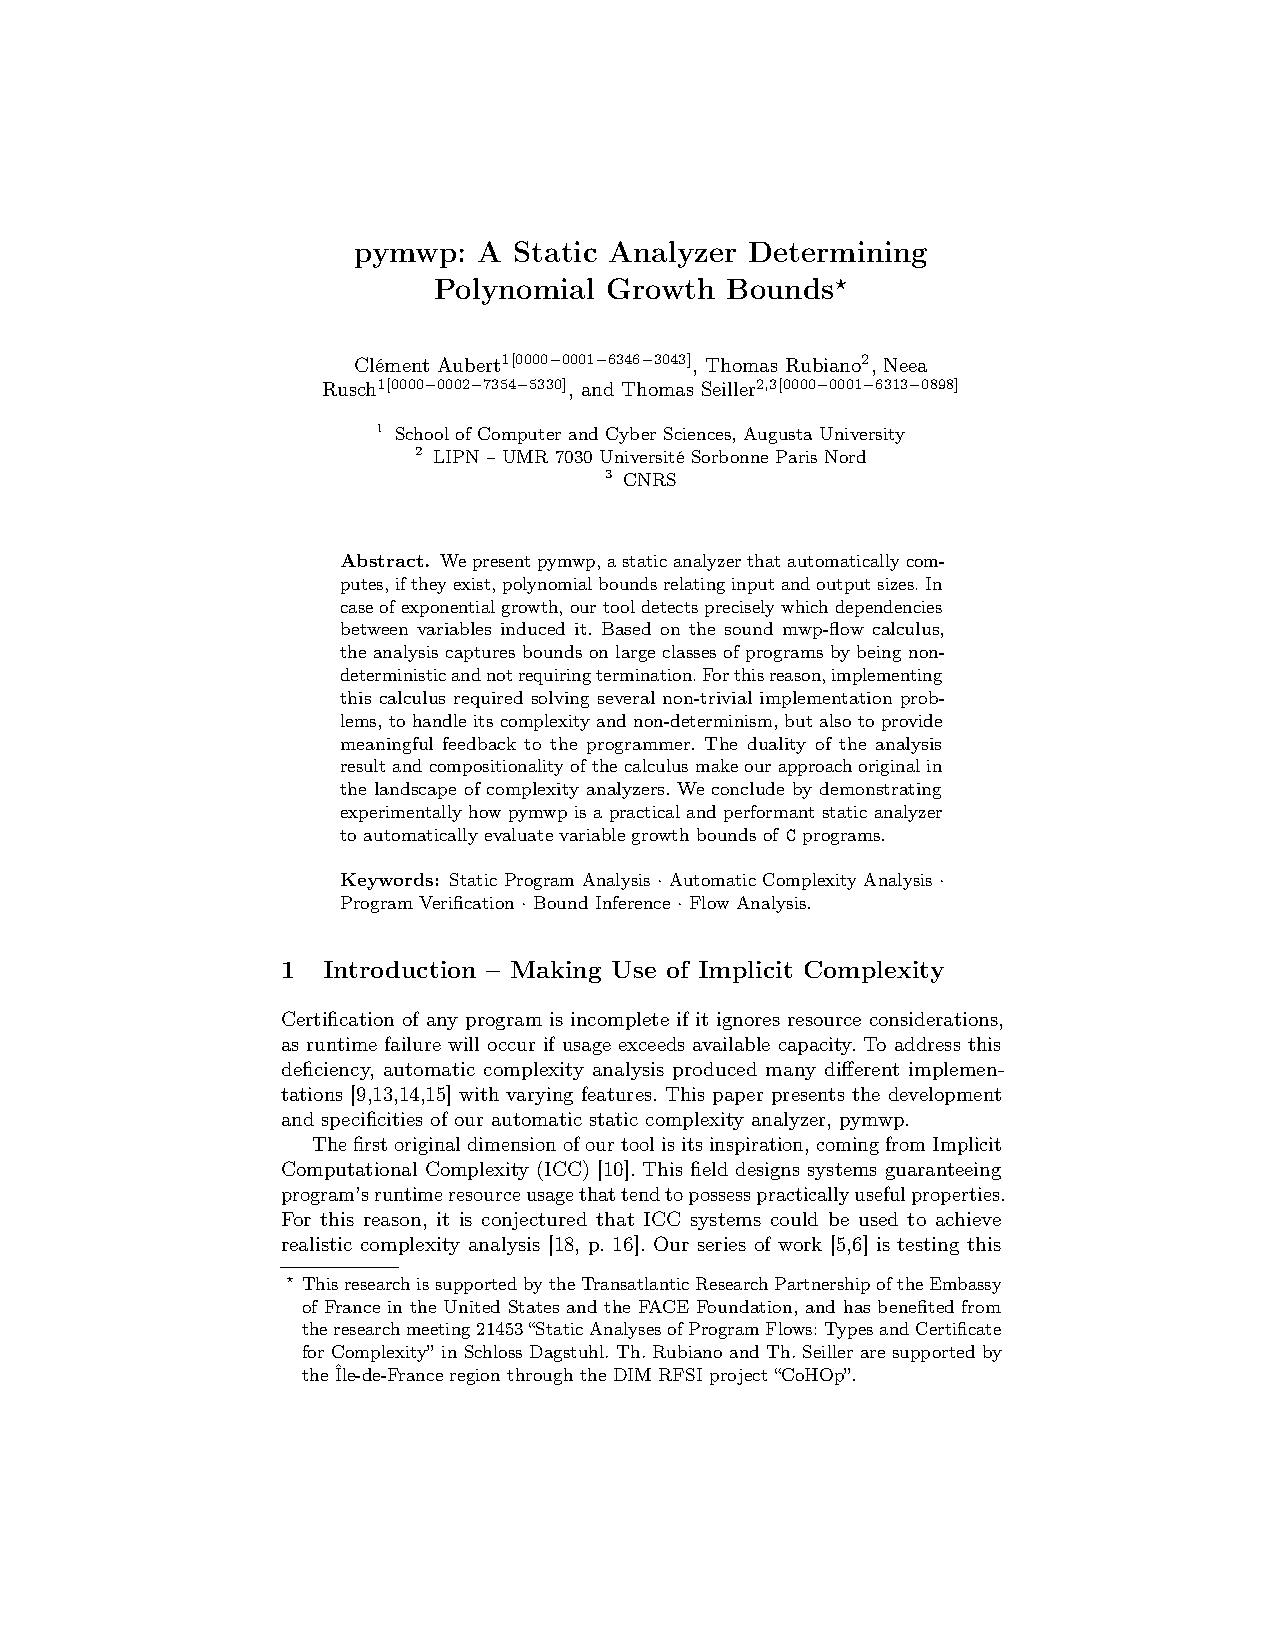
\includepdf[pages=-,pagecommand={\stepcounter{insertpages}},addtolist={
5,table,Comparison of obtained resource bounds.,tab:compare,
10,table,Benchmark results.,tab:eval,
10,table,Examples of obtained bounds.,tab:bounds
}]{papers/atva/main.pdf}

%----------------------------------------------------------------------------------------
%	3. UNPUBLISHED RESEARCH
%----------------------------------------------------------------------------------------
\chapter{Unpublished Research}\label{ch:unpublished-research}
% This can include manuscripts, in the journal format, that have been submitted for
% publication that are under review at the time of dissertation submission. Manuscripts
% that have been rejected or that have not been submitted (in preparation) cannot be
% included in the journal format (i.e. must conform to the traditional dissertation
% format). For manuscripts that have been submitted and are under review, the first
% authorship of the candidate must be maintained when the manuscript is published.

%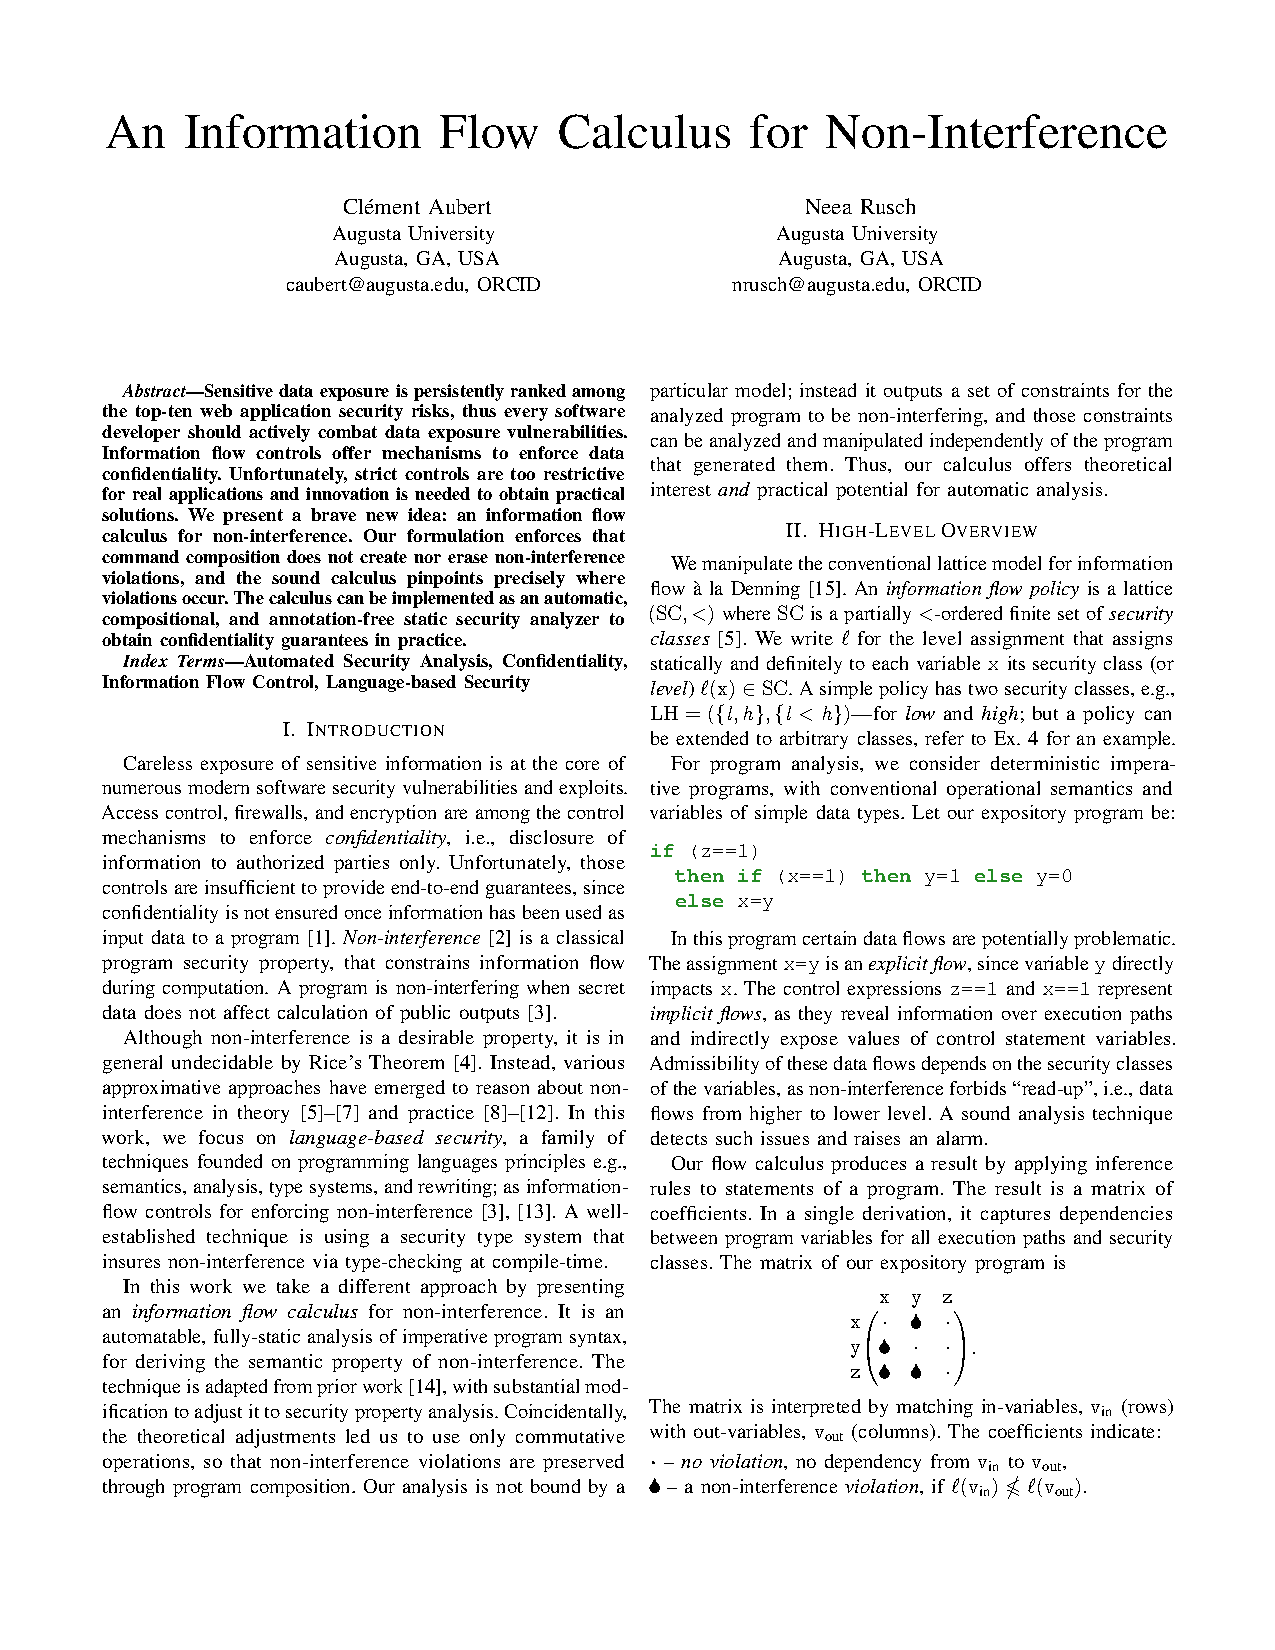
\includepdf[pages={1-},pagecommand={\thispagestyle{empty}\stepcounter{insertpages}
%\ifnum\value{insertpages}=1\addcontentsline{toc}{section}{
%An Information Flow Calculus for Non-Interference}\fi
%}]{papers/plas/main.pdf}\setcounter{insertpages}{0}

\clearpage\tocless\section{Motivation}

The ability to statically infer resource bounds of programs offers numerous benefits, \eg
to insure safe memory usage.
Even more preferable if those guarantees are established with the rigor of formal verification,
because that increases confidence in the obtained analysis result and enables integration of complexity
analyses into larger formal developments.

% Complexity with Coq is hard.
Unfortunately, computational complexity is notoriously difficult to represent formally for several reasons.
In general, deriving a complexity bound for an arbitrary program is an undecidable problem. % Address comment of review #2D here?
In the area of complexity theory, \textcquote[p.~114]{forster2020}{formalisations of even basic complexity-theoretic results are not available}, hindering certification attempts.

For practical complexity analyses, many existing techniques present methodological challenges if they require \eg program termination or inlining functions~\cite{carbonneaux2015}.
Therefore, a realistic pathway toward formal certification of a program's resource usage is narrow.
A few encouraging early results exist, and we discuss some of those in \autoref{coqpl-related}.
In this proposal we will sketch how a different approach, founded on Implicit Computational Complexity,
could sidestep some of the usual difficulties in implementing and verifying complexity analyses in Coq.

% ICC offers a way.
The field of Implicit Computational Complexity (ICC)~\cite{dallago2011} drives better understanding of complexity classes, but it
also guides the development of resources-aware languages and static source code analyzers.
The core idea is to bound resources \emph{while the program is being written (or type checked)} instead of measuring its resource usage afterwards on an abstract model of computation.
This can be done through \eg bounded recursion or using typing mechanisms.
The goal is to find a syntactical restriction or a type system such that a program can be written or typed only if it belongs to a particular complexity class.
ICC-based systems are often compositional and they offer more natural tools to write programs than theoretical models of computation used in complexity theory.
We speculate these combined properties could make ICC-approaches a conceivable pathway toward certified complexity and sketch a more detailed plan below.

\tocless\section{Preliminary Action Plan}  % Replace with a better title

We plan to formalize in Coq an ICC-based complexity analysis technique, the \emph{mwp-flow analysis}~\cite{jones2009}\footnote{Where mwp stands for \emph{m}aximum, \emph{w}eak polynomial and \emph{p}olynomial, representing increasing growth rates of variables values.}.
We chose this method because its internal mechanics has been recently studied~\cite{aubert20222}, and by our assessment, it seems suitable for formalization in Coq.
As for Coq, it seems like the ideal target language because of its existing libraries and preliminary work--some of which are discussed in \autoref{coqpl-related}--, most notably related to compilers~\cite{leroy2009}.

\tocless\subsection{Overview of \emph{mwp}-Flow Analysis}

% ICC offers a way of doing statyc analysis.
%This later view on complexity was used to design statyc analyzers of simple imperative programming languages.
%One of them, the \emph{mwp}-analysis~\cite{Jones2009}, uses matrices to record data flows between variables.
%If a variables depends \enquote{too strongly} on another, it risks to grow exponentially if used carelessly inside a loop, and the analysis detects it and flags it.
%As a result, a program can get assigned a type---a matrix---only if all the values in it are bounded by a polynomial in the inputs sizes.
The \emph{mwp}-flow analysis certifies polynomial bounds on the size of the values manipulated by
an imperative program.
While it does not ensure (or require) program termination, it provides a certificate guaranteeing that the program uses throughout its execution at
most a polynomial amount of space, and as a consequence that if it terminates, it will do so in polynomial time in the size of its inputs.

The analysis computes, for each program variable, a vector tracking how it depends on other variables.
The vector values are determined by applying the nondeterminitic rules of the sound \emph{mwp}-calculus to the commands of the program.
Those vectors are collected in a matrix.
A program is assigned a matrix only if all the values in it are bounded by a polynomial in the inputs sizes.
This technique is compositional, abstracts away \eg iteration bounds, and operates on
a memory-less imperative language, reminiscent of the \texttt{Imp} language from Software Foundations~\cite%[Imp:Simple Imperative Programs]
{cpierce20221}.

% Our plan
%This analysis offers many advantages compared to more traditional static analyzers: for instance, it is compositional, and returns a multi-variate growth bound, if one can be derived.
%It is also extremely fast, partly because it is not concerned with loop counters: the analysis is simply insensible to the loops' conditions.
%Those first encouraging results have been refined and implemented~\cite{pymwp,Aubert2022b,Aubert2022g,Aubert2022l}, and we believe they constitute an excellent path toward verifying resource bounds with Coq.

% What we have done.
%The original analysis~\cite{Jones2009} was computationally expensive and slow: our first efforts were geared toward, in parallel, stream-lining the theoretical construction~\cite{Aubert2022b} and implementing it~\cite{pymwp,Aubert2022l} to insure that our strategy was realistic.
%We are now in possession of a resilient and realistic static analyzer, whose correctness was reduced to the one of the original calculus~\cite{Jones2009}.
%We believe it is now time to certify this original calculus, whose main result states that a program can be assigned a matrix iff there is an honest polynomial bounding the growth-rate of its variables.

\tocless\subsection{The Coq Formalization}

Our goal is to certify the analysis as presented in the original paper~\cite{jones2009}.
Note that this does not mean that the bound is certified, but that \emph{the mechanism to compute those bounds} is certified.
Of course, this implies the correctness of the bounds as a by-product but constitutes a major difference \wrt the results discussed in \autoref{coqpl-related}.
%
Preliminary explorations have led us to establish the following milestones.

\begin{description}
\item[The mathematical foundations]
Our first goal is to define the mathematical structure required to carry out the rest of the construction.
This requires defining vectors, matrices and their operations, semi-rings, and honest polynomials\footnote{Which are \textcquote[p.~5]{jones2009}{polynomial build up from constants in $\mathbb{N}$ and variables by applying the operations $+$ (addition) and $\times$ (multiplication).}} that are
needed to represent the \emph{mwp}-bounds.
The Mathematical Components library~\cite{mahboubi2022} will lay the foundations for the linear algebra representations,
but likely requires extensions to accommodate our specific analysis.

\item[Implementing the language]
The analyzed language is a simple imperative language that manipulates natural numbers,
held in a fixed number of program variables. Its syntax includes
variables, expressions (operations $+$ and $\times$), Boolean expressions, and commands (\eg  assignment, loop and decision statements, command sequences, and skip), with their usual semantics.
We expect implementing it and its small-steps semantics in Coq to be relatively simple,
following the examples from Software Foundations~\cite{cpierce20221,cpierce20222}.

\item[Implementing the typing system]
Even if it can be computationally expensive to run an automatic inference~\cite{aubert2023b}, the typing system \emph{in itself} is relatively simple.
It contains only 10 rules, essentially one for each type of command, and except for the initial assignment of vectors to variables, is fully deterministic.
We conjecture that standard methods~\cite{chlipala2022, chlipala2010} to implement simple type systems will be enough, but will require some care to scale to the matrix-as-type paradigm of this analysis.

\item[Certifying the analysis]
This will be the most demanding part of our plan.
The original paper contains all the required handwritten proofs, but the authors caution that \enquote{\textins{t}hese proofs are long, technical and occasionally highly nontrivial}~\cite[p.~2]{jones2009}.
The main result of the paper is the soundness proof of the analysis~\cite[Theorem 5.3]{jones2009},
\ie the proof of the existence of a matrix typing the program implies the existence of an honest polynomial bounding the variables' growth rates.
The main result follows from 15 pages of proofs presented in section 7 of the paper.
This section revolves around proving the soundness properties of the calculus,
and we expect the most substantial effort to be spent on formalizing these proofs.
Some of them are quite intricate but with a satisfactory level of detail.
The cases concerning soundness of loops are the most difficult on paper, but their inductive nature \emph{should} (we hope!) be processed by Coq rather easily.%, in part because they require computing the fixpoint of matrices.
\end{description}

We leave for future work the possibility of creating a formally verified, automatic static analyzer founded on the proof of correctness of this method: as we discussed in other works~\cite{aubert2023b,aubert20222}, care is required to implement a typing strategy that does not rapidly become intractable.

\tocless\section{Related Work}\label{coqpl-related}

A few prior results exist that combine formalization of complexity and Coq.
They range from practical analyses to proofs in computational complexity theory.

For practical application, Coq has been used to verify stack bounds for assembly code~\cite{carbonneaux2014}
and to obtain WCET loop-bound estimation~\cite{blazy2013}.
Carbonneaux et al. ~\cite{carbonneaux2017} presented an automatic static analyzer for imperative programs, and although the analyzer itself is not verified, it generates bounds with machine-checkable certificates, to guarantee that the computed bound holds.
For functional paradigm, McCarthy et al.~\cite{mccarthy2018} developed a Coq library, with a monad that counts abstract steps, which enabled running time analysis of programs written using the monad.
An ICC-based characterization was introduced by F\'{e}r\'{e}e et al.~\cite{feree2018}, in the form of a
Coq library, that allows for readily proving that a function is computable in polynomial time. % Do something to clarify reviewer #2A here?

Coq has also been used to formalize some of the foundations of modern complexity theory.
Ciaffaglione~\cite{ciaffaglione2016} proved the undecidability of the halting problem.
Gu{\'e}neau et al.~\cite{gueneau2018} formalize the \(\mathcal{O}\) notation.
Forster et al.~\cite{forster2020} implemented a multi-tape to single-tape compiler, and
introduced the first formalized universal Turing Machine verified \wrt time and space complexity, for any model of computation, in any proof assistant.
More recently, G\"{a}her and Kunze formalized the Cook-Levin theorem in Coq~\cite{gaher2021}.
Despite these advances, formalization of complexity is in early stages and basic complexity-theoretic
results \eg time and space hierarchy theorems, remain unavailable.

Our proposed project differs from these earlier results primarily in its intent.
We plan to formalize the complexity analysis mechanism itself---not its computed result, as was done previously.
In their work with the Turing Machines, Forster et al.~\cite{forster2020} were explicit
in emphasizing the challenge they experienced in formalizing complexity.
We hypothesize that our ICC-based approach, with \eg its built-in abstractions, will help reduce this challenge.
It is our hope that CoqPL will welcome our proposal for a certified complexity analysis in Coq, and will be keen on indicating any library, tool or resource that could help.


%----------------------------------------------------------------------------------------
%	4. DISCUSSION
%----------------------------------------------------------------------------------------
\chapter{Discussion}\label{ch:discussion}
A comprehensive discussion that integrates the findings of all research presented
in the dissertation and that identifies how the goals or specific aims of the project
were attained, and how the research has answered the hypotheses put forth in the
dissertation.


%----------------------------------------------------------------------------------------
%	5. SUMMARY
%----------------------------------------------------------------------------------------
\chapter{Summary}\label{ch:summary}
A series of concise remarks summarizing experimental findings and conclusions

%----------------------------------------------------------------------------------------
%	6. REFERENCES
%----------------------------------------------------------------------------------------
\chapter{References}\label{ch:references}
% All literature cited in the dissertation will be included here. Style should conform
% to selected style manual. References included in manuscripts must be renumbered and
% reformatted (if needed) and included in this section. Literature Cited sections within
% the manuscripts should be omitted.
\printbibliography[heading=none,sorting=none]

%----------------------------------------------------------------------------------------
%	7. APPENDICES
%----------------------------------------------------------------------------------------
\chapter{Appendices}\label{ch:appendices}\clearpage

\section*{mwp-Analysis Improvement and Implementation: Realizing Implicit Computational Complexity}\label{sec:fscd}
\addcontentsline{toc}{section}{mwp-Analysis Improvement and Implementation: Realizing Implicit Computational Complexity}
\ainfo{Cl{\'{e}}ment Aubert, Thomas Rubiano, Neea Rusch, Thomas Seiller}{International Conference on Formal Structures for Computation and Deduction, 2022}
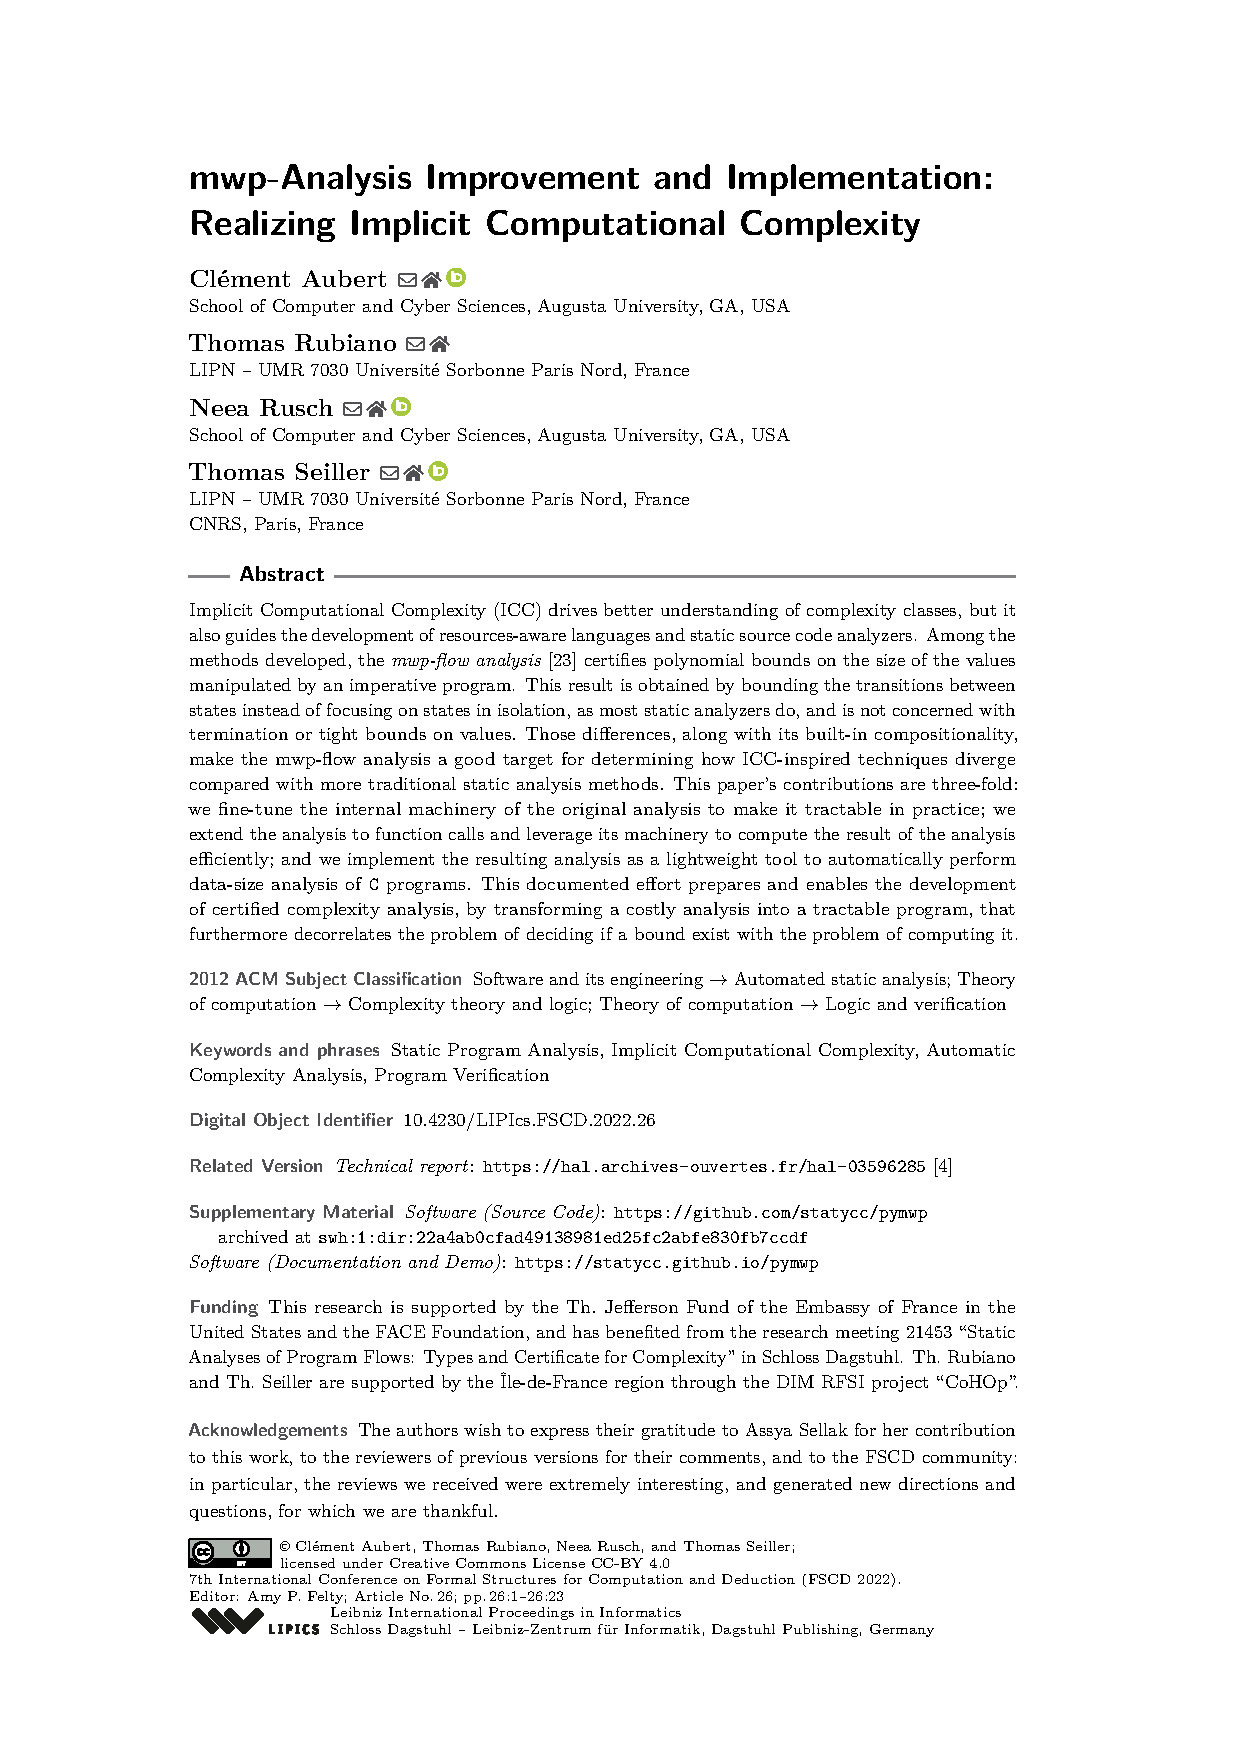
\includepdf[pages={1-},pagecommand={\thispagestyle{empty}\stepcounter{insertpages}}]
{res/pubs_fscd.2022.pdf}\setcounter{insertpages}{0}

\section*{Distributing and Parallelizing Non-canonical Loops}\label{sec:vmcai}
\addcontentsline{toc}{section}{Distributing and Parallelizing Non-canonical Loops}
\ainfo{Cl{\'{e}}ment Aubert, Thomas Rubiano, Neea Rusch, Thomas Seiller}
{International Conference on Verification, Model Checking, and Abstract Interpretation, 2023}
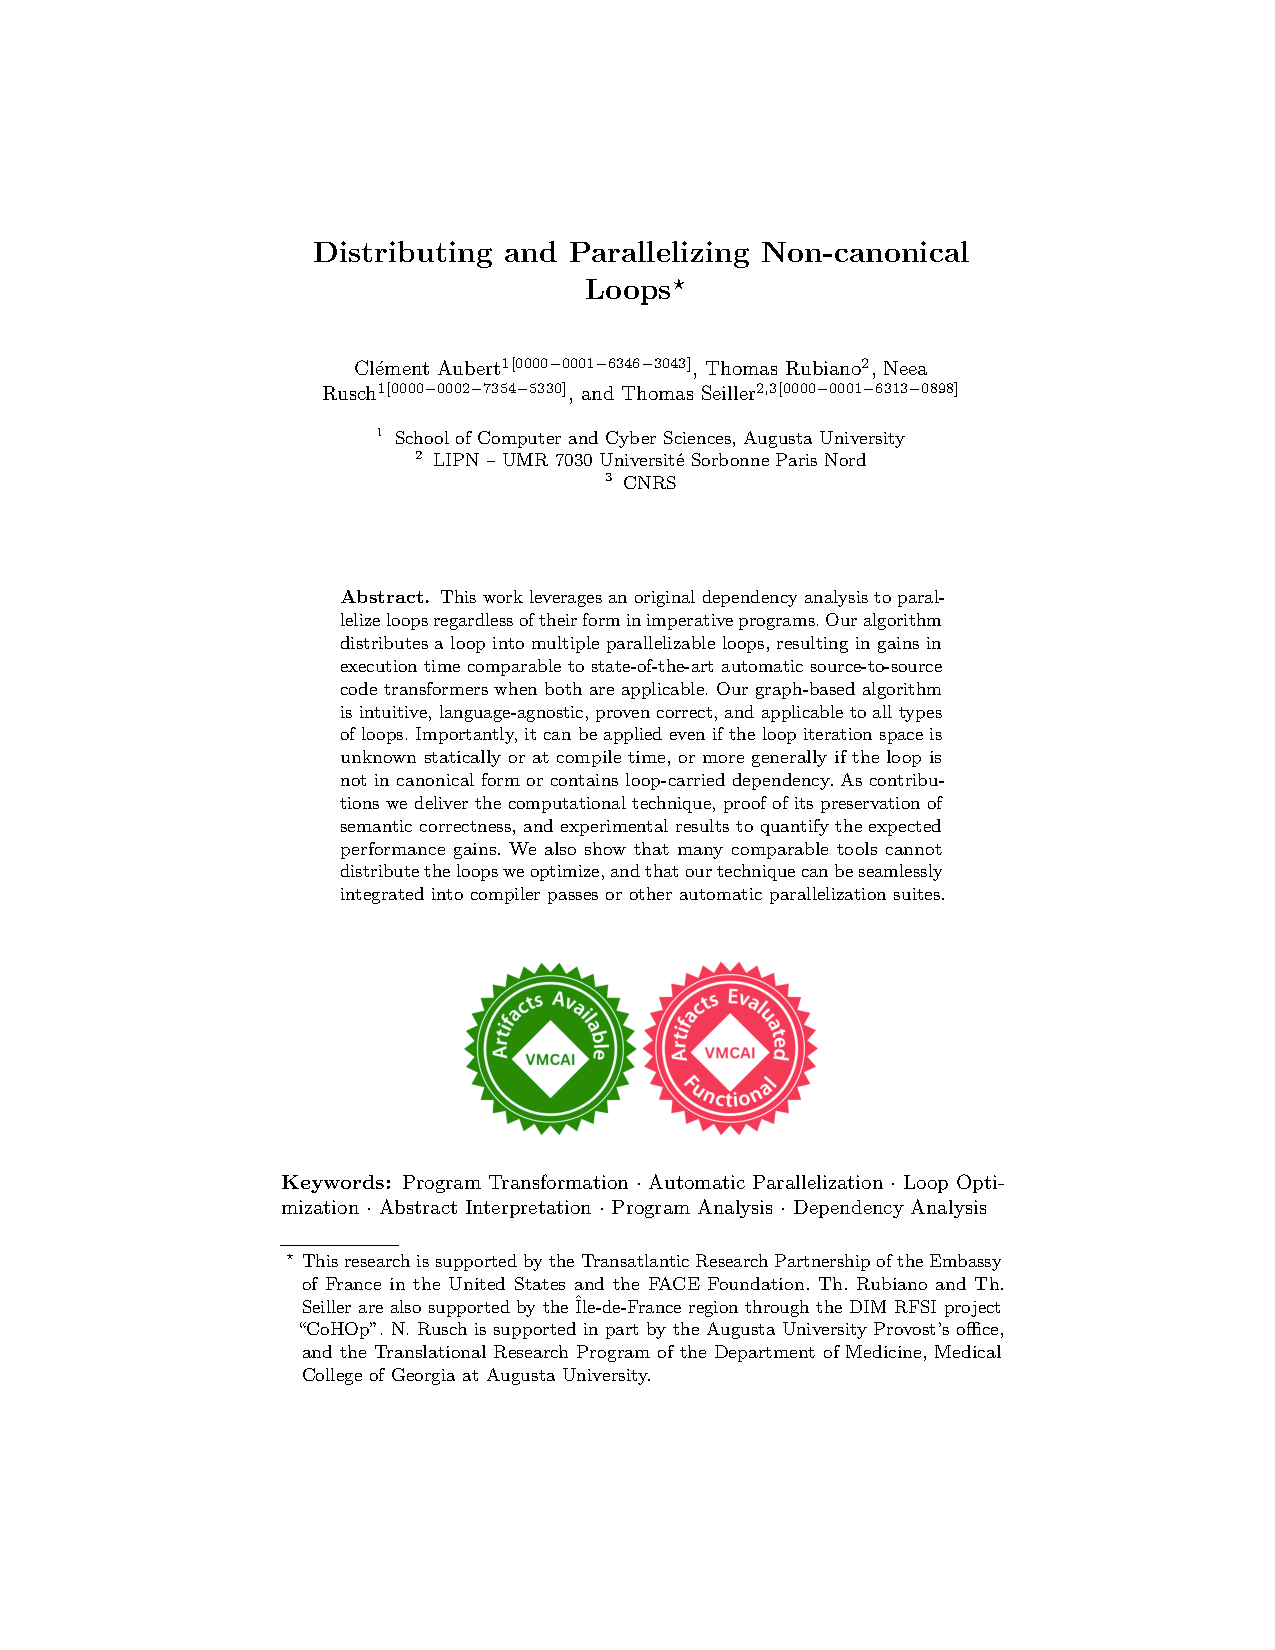
\includepdf[pages={1-},pagecommand={\thispagestyle{empty}\stepcounter{insertpages}}]
{res/pubs_vmcai.2023.pdf}\setcounter{insertpages}{0}

\section*{Tool User Guide for \enquote{pymwp: A Static Analyzer Determining Polynomial Growth Bounds}}\label{sec:tool-guide}
\addcontentsline{toc}{section}{Tool User Guide for \enquote{pymwp: A Static Analyzer Determining Polynomial Growth Bounds}}
\ainfo{Cl{\'{e}}ment Aubert, Thomas Rubiano, Neea Rusch, Thomas Seiller}
{A companion tool user guide}
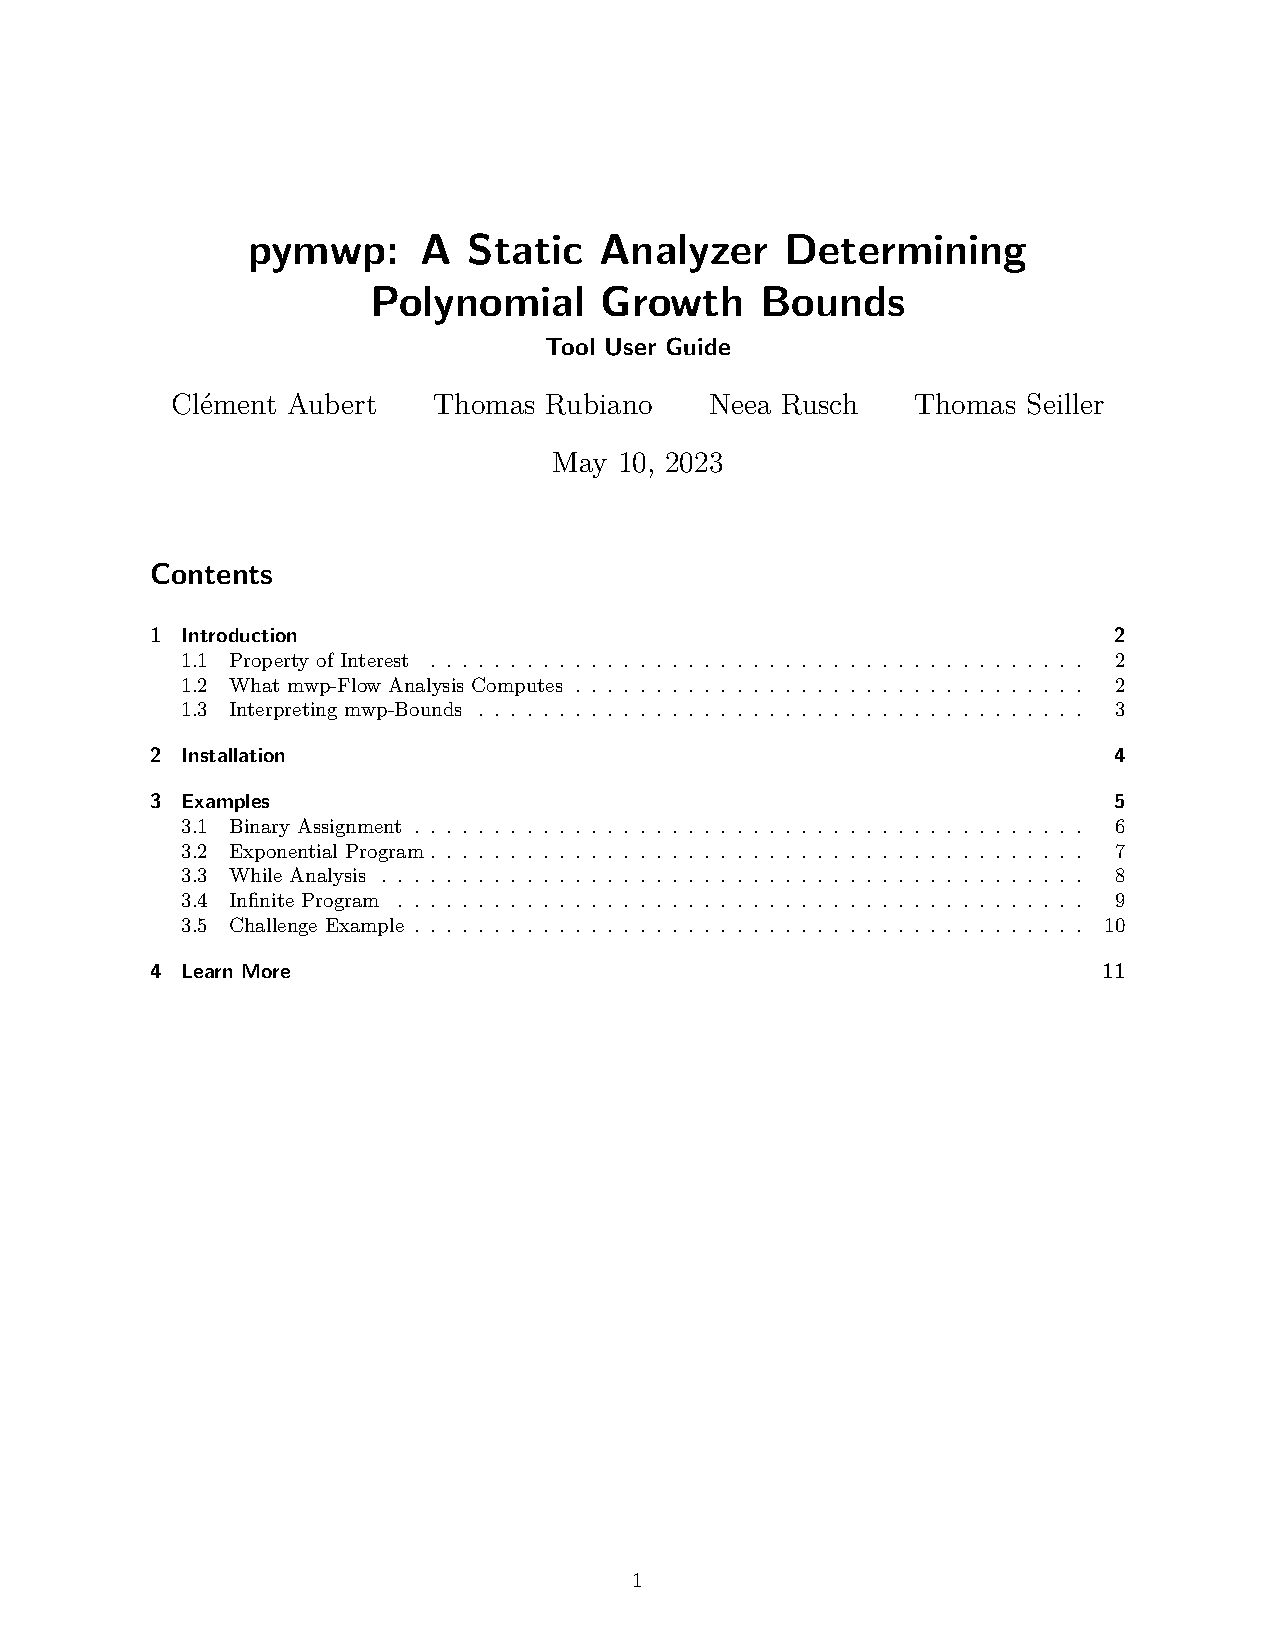
\includepdf[pages={1-},pagecommand={\thispagestyle{empty}\stepcounter{insertpages}}]
{res/pubs_pymwp_guide.pdf}\setcounter{insertpages}{0}

\end{document}